\documentclass{ieeeojies}
\usepackage{cite}
\usepackage{amsmath,amssymb,amsfonts}
\usepackage{algorithmic}
\usepackage{graphicx}
\usepackage{textcomp}
\usepackage{array}
\usepackage[table]{xcolor}
\usepackage{multirow}
\usepackage{multicol}
\usepackage{float}
\usepackage{enumitem}
\usepackage{amsmath}
\usepackage{breqn}

\def\BibTeX{{\rm B\kern-.05em{\sc i\kern-.025em b}\kern-.08em
    T\kern-.1667em\lower.7ex\hbox{E}\kern-.125emX}}

\begin{document}
\title{UTILIZING STATISTICAL MODEL & MACHINE LEARNING FOR VIETNAMESE STOCK PRICE FORECASTING}

\author{\uppercase{DUONG CHI TAM NGUYEN}\authorrefmark{1},
\uppercase{HIEN THAO DO\authorrefmark{2}, and MANH HUY HUYNH}\authorrefmark{3}}

\address[1]{Faculty of Information Systems, University of Information Technology, (e-mail: 21520439@gm.uit.edu.vn)}
\address[2]{Faculty of Information Systems, University of Information Technology, (e-mail: 21520460@gm.uit.edu.vn)}
\address[3]{Faculty of Information Systems, University of Information Technology, (e-mail: 21520259@gm.uit.edu.vn)}

\markboth
{Author \headeretal: DUONG CHI TAM NGUYEN, HIEN THAO DO, MANH HUY HUYNH}
{Author \headeretal: DUONG CHI TAM NGUYEN, HIEN THAO DO, MANH HUY HUYNH}

\begin{abstract}
\\In recent years, stock trading has always been a significant part of the financial world. With the potential of the stock market and the rapid development of machine learning, stock prices prediction has been a hot issue. Investors can reduce potential losses, make informed investment decisions and promote development by using forecast tool. In this study, we will use Statistical Model and Machine Learning Algorithms such as Linear Regression, ARIMA, RNN, GRU, LSTM, AR-MOS, Random Forest, Neural Hierarchical Interpolation for Time Series Forecasting (N-HiTS) to forecast the stock prices of three corporations in Vietnam.
\end{abstract}

\begin{keywords}
\\Stock price forecasting, autoregressive adjusted model output statistics (AR-MOS),  Linear Regression, ARIMA, RNN, GRU, LSTM, Random Forest, Neural Hierarchical Interpolation for Time Series Forecasting (N-HiTS), Time series analysis, Predictive analytics.
\end{keywords}

\titlepgskip=-15pt

\maketitle

\section{Introduction}
\label{sec:introduction}
 \indent A stock market is a public market where you can buy and sell shares for publicly listed companies. The stocks represent ownership in the company. The stock exchange is the mediator that allows the buying and selling of shares. Stock Price Prediction using machine learning algorithm helps to discover the future value of company stock and other financial assets traded on an exchange. [1]\\
 \indent Vietnam’s stock market has experienced significant growth in recent years. However, forecasting stock prices in this market remains a challenging due to the complexities of financial market. There are other factors involved in the prediction, such as physical and psychological factors, rational and irrational behavior, and so on. All these factors combine to make share prices dynamic and volatile. This makes it very difficult to predict stock prices with high accuracy [1]. In order to analyze and make predictions about financial data, particularly stock prices, machine learning techniques have become increasingly effective. \\
 \indent In this study, we especially focus on applying machine learning algorithms to forecast stock values on three corporations in Vietnam: Vietnam Dairy Products JSC (VNM), Saigon Beer Alcohol Beverage Corp (SAB), Masan Group Corp (MSN). By employing machine learning such as Random Forest, AR-MOS, N-HiTS, …; this research seeks to enhance the accuracy and reliability of stock price prediction, enabling stakeholders in Vietnam's stock market to make well-informed investment decisions.
\section{Related Works}
\indent In recent years, there has been a substantial amount of research dedicated to predicting stock prices using various machine learning and statistical models.\\
\indent V. Gururaj, in a 2019 study [2], focused on stock market prediction employing Linear Regression and Support Vector Machines, demonstrating the application of these models in forecasting stock prices.\\
\indent Zhong and Enke in 2019. Predicting the daily return direction of the stock market using hybrid machine learning algorithms. For evaluating a classification model’s accuracy, recall, precision, and F-score, are commonly preferred metrics, and for regression or price forecasting models, root mean square error (RMSE) and mean absolute percentage error (MAPE) are often employed. Jose el at. in 2019 An Efficient System to Predict and Analyze Stock Data using Hadoop Techniques.

\section{Materials}
\subsection{Dataset}

We collected three datasets on Investing.com from March 1, 2019 to June 4, 2024. The data related to stock price of three large companies in Vietnam:  Vietnam Dairy Products JSC (VNM), Saigon Beer Alcohol Beverage Corp (SAB), Masan Group Corp (MSN). The dataset has 7 attribute columns including: Date, Price, Open, High, Low, Vol, Change. As the goal is
to forecast close prices, only data relating to column “Price"
(VND) will be processed.

\subsection{Descriptive Statistics}
\begin{table}[H]
  \centering
  \caption{MSN, SAB, VNM’s Descriptive Statistics}
\begin{tabular}{|>{\columncolor{red!20}}c|c|c|c|}
    \hline
     \rowcolor{red!20} & MSN & SAB & VNM \\ \hline
     Count & 1315 & 1315 & 1315 \\ \hline
     Mean & 82289.35 & 144544.26 & 82217.51\\ \hline
     Std & 23370.05 & 67194.6 & 13608.46\\ \hline
     Min & 39997 & 52500 & 58115.3\\ \hline
     25\% & 68000 & 80066.5 & 69935.6\\ \hline
     50\% & 78400 & 150150 & 80151.1\\ \hline
     75\% & 96159 & 180779 & 95539.25\\ \hline
     Max & 142286 & 289000 & 111828\\ \hline
\end{tabular}
\end{table}

\begin{figure}[H]
    \centering
    \begin{minipage}{0.23\textwidth}
    \centering
    \includegraphics[width=1\textwidth]{BoxPlotofMSN.png}
    \caption{MSN stock price's boxplot}
    \label{fig:1}
    \end{minipage}
    \hfill
    \begin{minipage}{0.23\textwidth}
    \centering
    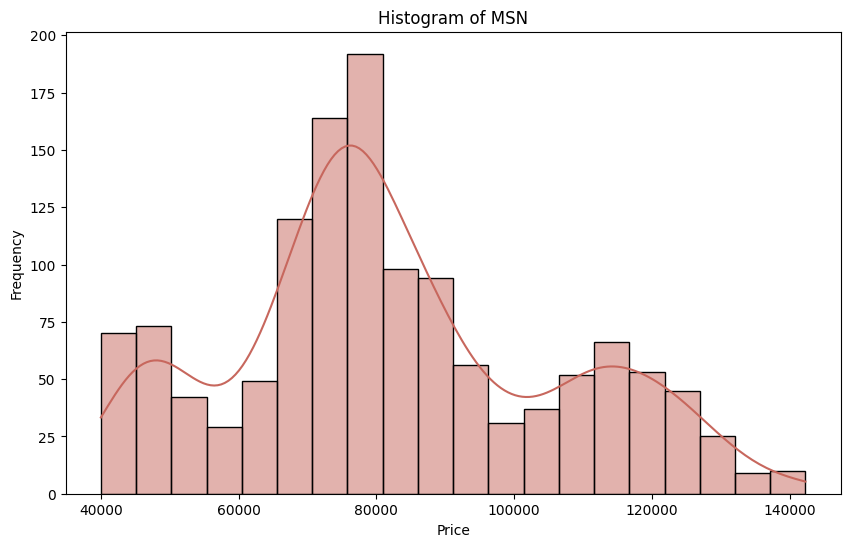
\includegraphics[width=1\textwidth]{HistogramOfMSN.png}
    \caption{MSN stock price's histogram}
    \label{fig:2}
    \end{minipage}
\end{figure}

\begin{figure}[H]
    \centering
    \begin{minipage}{0.23\textwidth}
    \centering
    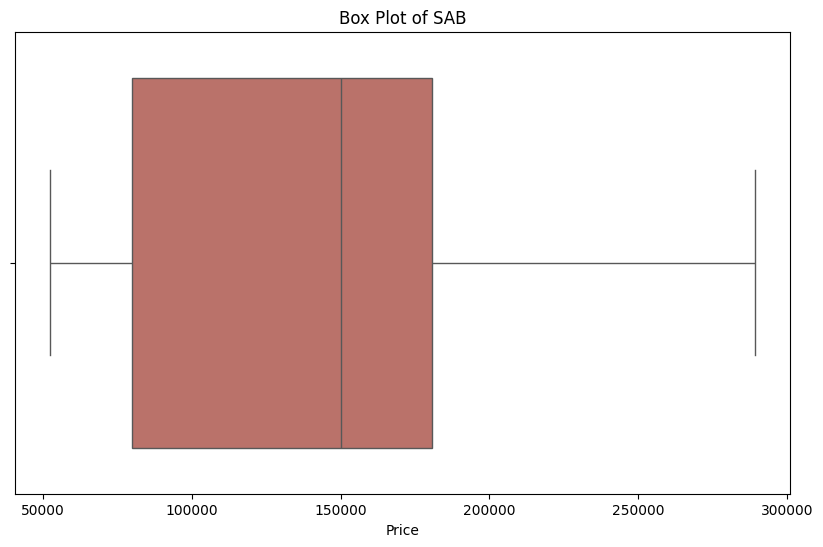
\includegraphics[width=1\textwidth]{BoxPlotOfSAB.png}
    \caption{SAB stock price's boxplot}
    \label{fig:1}
    \end{minipage}
    \hfill
    \begin{minipage}{0.23\textwidth}
    \centering
    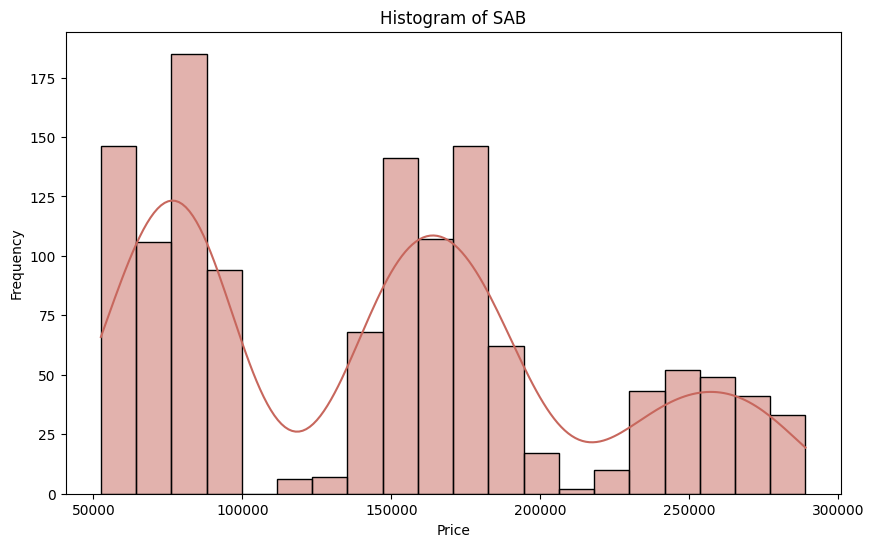
\includegraphics[width=1\textwidth]{HistogramOfSAB.png}
    \caption{SAB stock price's histogram}
    \label{fig:2}
    \end{minipage}
\end{figure}

\begin{figure}[H]
    \centering
    \begin{minipage}{0.23\textwidth}
    \centering
    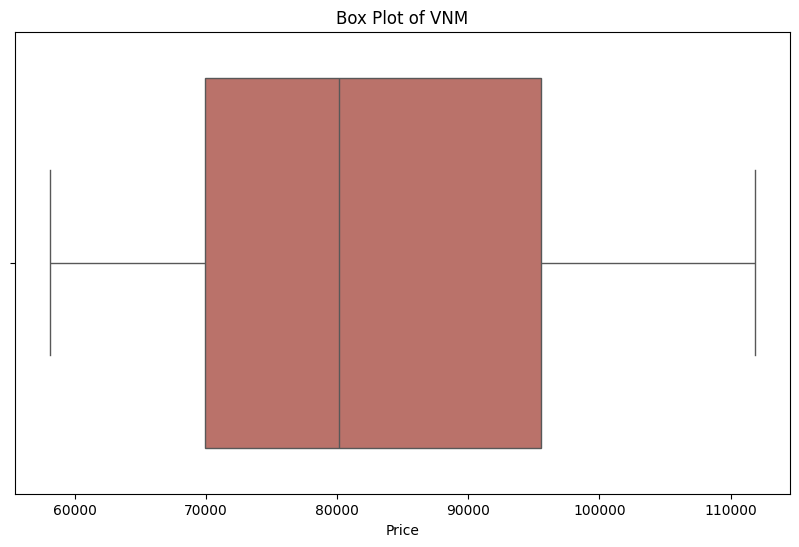
\includegraphics[width=1\textwidth]{BoxPlotOfVNM.png}
    \caption{VNM stock price's boxplot}
    \label{fig:1}
    \end{minipage}
    \hfill
    \begin{minipage}{0.23\textwidth}
    \centering
    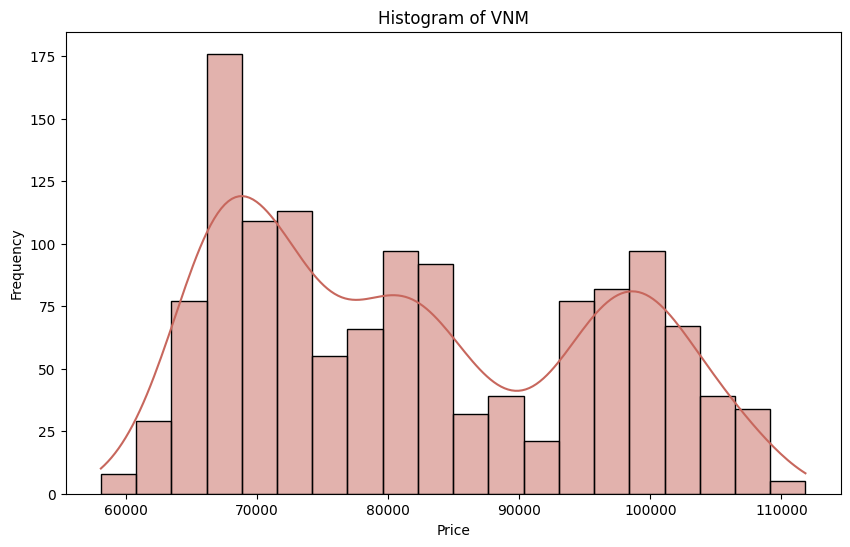
\includegraphics[width=1\textwidth]{HistogramOfVNM.png}
    \caption{VNM stock price's histogram}
    \label{fig:2}
    \end{minipage}
\end{figure}

\section{Methodology}
\subsection{Arima}
\indent An autoregressive integrated moving average, or ARIMA, is a statistical analysis model that uses time series data to either better understand the data set or to predict future trends [3]. The ARIMA model incorporates three key elements from the Box-Jenkins method: Autoregressive (AR), Integrated (I) – uses differencing of raw observations to make the time series stationary, Moving Average (MA).

[5][6] ARIMA model is classified as an ARIMA(p,d,q) model, where:
\begin{itemize}
    \item p is the order of AR term; indicates the number of lagged orders considered in the model.
    \item d defines the number of difference to make series stationary.
    \item q is the order of MA term; represents the number of lagged forecast errors in the prediction equation.
\end{itemize}
The formula to denote the AR is shown:
\[ Y_t = c + \phi_1 Y_{t-1} + \phi_2 Y_{t-2} +...+ \phi_p Y_{t-p} + \epsilon_t\]
Which t is the time series so \(Y_t\) is the value of the time series at time t; p is used to calculate the number of orders of previous values; \(\phi\) is the autoregressive coefficients; \(\epsilon_t\) is the error term. The expected value is zero. 
The formula to denote the AR is shown:
\[ Y_t = c + \epsilon_t + \theta_1 \epsilon_{t-1} + \theta_2 \epsilon_{t-2} +...+ \theta_p  \epsilon_{t-p}\]
Where q denotes the quantity of orders required to locate the historical values, is used to specify how many orders are included in the AR computation. If we combine differencing with the autoregression and the moving average model, the ARIMA(p, d, q) can be written as:
\[ Y'_t = c + \phi_1 Y'_{t-1} +...+ \phi_p Y'_{t-p} + \theta_1 \epsilon_{t-1} +...+ \theta_p  \epsilon_{t-p} + \epsilon_t\]
Where \(Y'_t\) is the differenced series; the “predictors” on the right hand side include both lagged values of  \(Y_t\) and lagged errors.
\subsection{Linear Regression}
Linear regression is used to predict the value of a variable based on the value of another variable. The variable need to predict is called the dependent variable. The variable that is used to predict the other variable's value is called the independent variable. Linear regression fits a straight line or surface that minimizes the discrepancies between predicted and actual output values. [7] \\
A multiple linear regression model has the formula as below: [8]
\[ Y = \beta_0 + \beta_1X_1 + \beta_2X_2 +...+ \beta_nX_n + \epsilon\]
Where:
\begin{itemize}
    \item $Y$ is the dependent or predicted variable.
    \item $\begin{aligned}[t]
            X_1,...X_n & \text{ are the independent (explanatory) variables.} \\
            \end{aligned}$
    \item $\begin{aligned}[t]
            \beta_0 & \text{ is the intercept term.} \\
            \end{aligned}$
    \item $\begin{aligned}[t]
            \beta_1,...\beta_n & \text{ are the regression coefficients for the independent variables.} \\
            \end{aligned}$
    \item $\begin{aligned}[t]
            \epsilon & \text{ is the random error.}
            \end{aligned}$        
\end{itemize}
\subsection{AR-MOS}
\indent AR-MOS (Auto-Regressive Model Output Statistics) is a method that combines the auto-regressive (AR) model and MOS (Model Output Statistics) to improve the accuracy of weather forecasts. By integrating these methods, AR-MOS corrects systematic errors in numerical weather prediction models and utilizes past forecast data to enhance the accuracy of future predictions. 
\indent Autoregressive models (AR) belong to time series models. These models capture the relationship between an observation and several lagged observations (previous time steps). The core idea is that the current value of a time series can be expressed as a linear combination of its past values, with some random noise.[9]

\indent Mathematically, an autoregressive model of order p, denoted as AR(p), can be expressed as:
\begin{dmath*}
 Y_t = c + \phi_1 Y_{t-1} + \phi_2 Y_{t-2} +...+ \phi_p Y_{t-p} + \epsilon_t 
 \end{dmath*}

Which t is the time series so \(Y_t\) is the value of the time series at time t; p is used to calculate the number of orders of previous values; \(\phi\) is the autoregressive coefficients; \(\epsilon_t\) is the error term.

\indent Model Output Statistics (MOS) is a method for improving weather forecasts by combining information from numerical weather prediction models with actual observational data. 
AR-adjusted forecast ensemble obtained via : 

\[\widetilde{x_i}(t) := x_i(t) + \widehat{r_i}(t) = x_i(t) + \eta_i + \sum_{j=1}^{p_k} \tau_{k,j} ( \widehat{r_i}(t - j) - \eta_k)
\]
With \(\eta_k, \tau_{k,j} \in \mathbb{R}\), \(j = 1, \ldots, p_k\) AR(\(p_i\)) coefficients, \(\widehat{r_i}(t)\),
\(i = 1, \ldots, m\) residuals obtained from \(y(t - j)\).

Predictive mean (location) estimated via
\[
\mu(t) := \frac{1}{m} \sum_{k=1}^{m} \widetilde{x_i}(t),
\]

Predictive variance (scale) via
\[
\sigma(t) := \omega \sigma_1(t) + (1 - \omega) \sigma_2(t).
\]

\(\sigma_1(t)\) is defined as:
\[
\sigma_1(t) := \sqrt{\frac{1}{m} \sum_{k=1}^{m} \gamma_k^2(t)},
\]
where \(\gamma_k^2(t)\) is the empirical variance of the AR(\(p_k\)) process.

\(\sigma_2(t)\) is the empirical standard deviation of the AR-adjusted forecasts \(\widetilde{x_i}(t)\),

\(\omega \in [0, 1]\) is a weight obtained by minimizing the Continuous Ranked Probability Score (CRPS) of the predictive Gaussian distribution. [19]

\subsection{Random Forest}
\indent Random Forest is a popular machine learning algorithm that belongs to the supervised learning technique. It can be used for both Classification and Regression problems in machine learning. It is based on the concept of ensemble learning, which is a process of combining multiple classifiers to solve a complex problem and to improve the performance of the model [20].
\indent Random forest algorithm combines the output from multiple decision trees to get a single result. It has three main hyperparameters, which need to be set before training. These include node size, the number of trees, and the number of features sampled. From there, the random forest classifier can be used to solve for regression or classification problems [11]. 

\begin{figure}[H]
    \centering
    \begin{minipage}{0.5\textwidth}
        \centering
        \includegraphics[width=1.0\textwidth]{Random Forest.png}
    \end{minipage}
\end{figure}
[10] The following steps explain the working Random Forest Algorithm:
\begin{enumerate}
  \item Select random samples from the given data or training set.
  \item Individual decision trees are constructed for each sample.
  \item Each decision tree will generate an output.
  \item Finally, the output is considered based on Majority Voting/Averaging.
\end{enumerate}
\indent Random Forest can also be used in time series analysis and forecasting, both univariate and multivariate dataset by creating lag variables and seasonality variables manually. When evaluating the performance of a Random Forest model, metrics such as standard deviation, var, moving average, and linear regression can provide insights into its effectiveness [21]. To implement Random Forest for time series forecasting, we need to [22]:
\begin{enumerate}
  \item Data Preparation: Convert the data into a suitable format.
  \item Data Splitting: Split into training and test sets. Ensure that the time order is preserved to avoid data leakage.
  \item Model Building: Fit the Random Forest model to the training data.
  \item Prediction: Make predictions using the trained model and evaluate its performance on the test set.
  \item Model Evaluation and Visualization.
\end{enumerate}
\subsection{RNN}
\indent Recurrent Neural Network(RNN) is a type of Neural Network where the output from the previous step is fed as input to the current step. In traditional neural networks, all the inputs and outputs are independent of each other.[12] RNNs differ from traditional feedforward neural networks in that they maintain a "hidden state" which contains information about previous elements in the sequence. This hidden state is updated at each time step t based on the input at that time and the hidden state from the previous time step.
\begin{figure}[H]
    \centering
    \begin{minipage}{0.23\textwidth}
    \centering
    \includegraphics[width=1\textwidth]{Simple RNN.png}
    \caption{Simple Recurrent Neural Network [13]}
    \label{fig:1}
    \end{minipage}
\end{figure}
A Neural Network usually include 3 specific layers as :
\begin{itemize}
    \item \textbf{Input layer (\(X_t\)): } The value input at time t.
\end{itemize}
\begin{itemize}
    \item \textbf{Hidden layer (\(H_t\)):  } The value containing the state information at time t.
\end{itemize}
\begin{itemize}
    \item \textbf{Output (\(Y_t\)):  } The value output at time t.
\end{itemize}

At any given time t, the current input is a combination of input at \(X_t\) and \(X_{t-1}\). The output at any given time is fetched back to the network to improve on the output. [13]


 \begin{figure}[H]
    \centering
    \begin{minipage}{0.50\textwidth}
    \centering
    \includegraphics[width=1\textwidth]{Fully connected RNN.png}
    \caption{Fully connected Recurrent Neural Network [14]}
    \label{fig:1}
    \end{minipage}
\end{figure}
Formula of the algorithm:
\[h_{(t)}\ =\ f_c(h_{(t-1)}\ ,\ x_{(t)})\]
Where : 
\begin{itemize}
    \item 	\(h_t\): new state.
\end{itemize}
\begin{itemize}
     \item \(h_t\): old state.
 \end{itemize}
 \begin{itemize}
     \item \(f_c\): function with parameter c .
 \end{itemize}

\begin{itemize}
    \item\(x_t\): input vector at time step t.
\end{itemize}


\subsection{LSTM}
LSTM networks are an extension of recurrent neural networks (RNNs) mainly introduced to handle situations where RNNs fail. [15] Unlike traditional RNNs, LSTM networks have a more complex structure with additional components called gates, which control the flow of information through the network. These gates include the input gate, forget gate, and output gate, each of which serves a specific purpose in managing the information flow. LSTM have been successfully used in a variety of tasks such as speech recognition, natural language processing, image captioning, and video analysis, among others. 
 \begin{figure}[H]
    \centering
    \begin{minipage}{0.50\textwidth}
    \centering
    \includegraphics[width=1\textwidth]{The LSTM structure.jpg}
    \caption{The LSTM cell structure.}
    \label{fig:1}
    \end{minipage}
\end{figure}
The cells store information, whereas the gates manipulate memory. There are three entrances:[16]
\begin{itemize}
    \item  \textbf{Input Gate:}  It determines which of the input values should be used to change the memory. The sigmoid function determines whether to allow 0 or 1 values through. And the tanh function assigns weight to the data provided, determining their importance on a scale of -1 to 1 . 
\end{itemize}
\[i_t = \sigma(W_i \cdot [h_{t-1}, x_t] + b_i)\]
\[C_t = tanh(W_c \cdot [h_{t-1}, x_t] + b_c)\]

\begin{itemize}
    \item  \textbf{Forget Gate: }  It finds the details that should be removed from the block. It is decided by a sigmoid function. For each number in the cell state Ct-1, it looks at the preceding state (ht-1) and the content input (\(x_t\)) and produces a number between 0 (omit this) and 1 (keep this).
\end{itemize}
\[f_t = \sigma(W_f \cdot [h_{t-1}, x_t] + b_f)\]
\begin{itemize}
    \item  \textbf{Output Gate }  The block’s input and memory are used to determine the output. The sigmoid function determines whether to allow 0 or 1 values through. And the tanh function determines which values are allowed to pass through 0, 1. And the tanh function assigns weight to the values provided, determining their relevance on a scale of -1 to 1 and multiplying it with the sigmoid output.
\end{itemize}
\[o_t = \sigma(W_o \cdot [h_{t-1}, x_t] + b_o)\]
\[h_t = o_t \cdot \tanh(C_t)\]
where: 
\begin{itemize}
    \item \(\sigma\) : is the sigmoid activation function.
    
\end{itemize}
\begin{itemize}
    \item \(i_t\),\(f_t\), \(o_t\) are the input, forget, and output gate vectors, respectively.  
\end{itemize}
\begin{itemize}
    \item W and b are the corresponding weight matrices and bias vectors.
\end{itemize}
\begin{itemize}
    \item \(h_t\) : is the hidden state/output at time t.
\end{itemize}
\begin{itemize}
    \item \([h_{t-1}, x_t]\): denotes the concatenation of the previous hidden state and the current input.
\end{itemize}
\begin{itemize}
    \item \(x_t\): is the input at time t.
\end{itemize}
\begin{itemize}
    \item \(C_t\): is the cell state at time t.
\end{itemize}
\subsection{GRU}
A Gated Recurrent Unit (GRU) is a type of recurrent neural network (RNN) architecture that is used in the field of deep learning. GRUs are particularly effective for processing sequences of data for tasks like time series prediction, natural language processing, and speech recognition. They address some of the shortcomings of traditional RNNs, particularly issues related to long-term dependencies in sequence data.[17]

GRU is to use gating mechanisms to selectively update the hidden state of the network at each time step. The gating mechanisms are used to control the flow of information in and out of the network. The GRU has two gating mechanisms, called the reset gate and the update gate. [18] The update gate determines how much of the past information needs to be passed along to the future. The reset gate decides how much of the past information to discard.
\begin{figure}[H]
    \centering
    \begin{minipage}{0.30\textwidth}
    \centering
    \includegraphics[width=1\textwidth]{Gated Recurrent Unit’s architecture.png}
    \caption{Gated Recurrent Unit’s architecture}
    \label{fig:1}
    \end{minipage}
\end{figure}
The equations used to calculate the reset gate, update gate, and hidden state of a GRU are as follows [18]:
\begin{itemize}[label={--}]
    \item \textbf{Update gate:} \[z_t = \sigma(W_z \cdot [h_{t-1}, x_t])\]
    \item \textbf{Reset gate:} \[r_t = \sigma(W_r \cdot [h_{t-1}, x_t])\]
    \item \textbf{Candidate Hidden State:} \[h'_t = \tanh(W \cdot [r_t \cdot h_{t-1}, x_t] + b)\]
    \item \textbf{Final Hidden State:}  \[h_t = (1 - z_t) \cdot h_{t-1} + z_t \cdot h'_t\]
\end{itemize}
Where: 
\begin{itemize}
    \item $\begin{aligned}[t]
            W_z, W_t, W & \text{ are weight matrices.} \\
            \end{aligned}$
    \item $\begin{aligned}[t]
            x_t & \text{ is the current input.} \\
            \end{aligned}$
    \item $\begin{aligned}[t]
            h_{t-1} & \text{ is the previous hidden state.} \\
            \end{aligned}$
   \item $\begin{aligned}[t]
            h_t & \text{ is the current hidden state.} \\
            \end{aligned}$     
    \item $b$ represents the bias.
\end{itemize}

\subsection{N-HiTS}
The Neural Hierarchical Interpolation for Time Series Forecasting (N-HiTS) is a deep learning algorithm designed for time series forecasting, addressing challenges in long-horizon predictions and capturing complex data patterns. It builds on concepts from the N-BEATS architecture, using local nonlinear projections onto basis functions through multiple blocks.
\begin{figure}[H]
    \centering
    \begin{minipage}{0.50\textwidth}
    \centering
    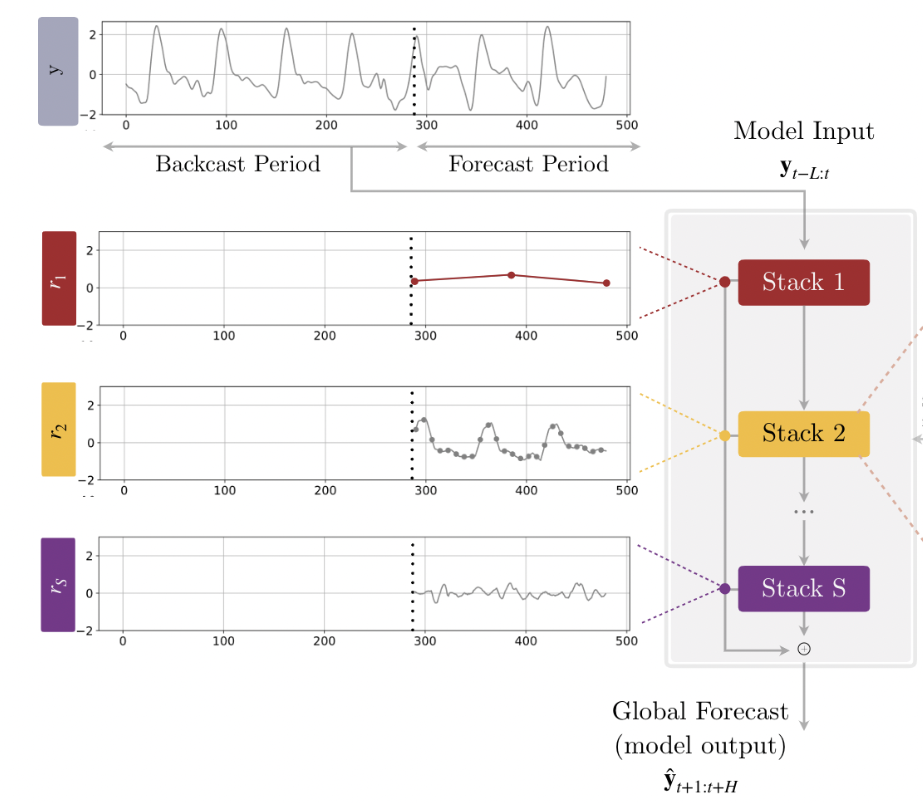
\includegraphics[width=1\textwidth]{N-HiTS Model Input.png}
    \caption{N-HiTS’s Model Input}
    \label{fig:1}
    \end{minipage}
    \begin{minipage}{0.50\textwidth}
    - Input Data is a Time Series \( y \) is divided into two parts: Backcast Period and Forecast Period.
    \end{minipage}
\end{figure}
\begin{figure}[H]
    \centering
    \begin{minipage}{0.15\textwidth}
    \centering
    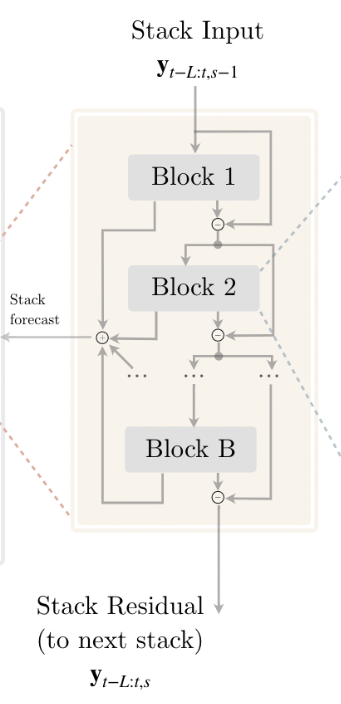
\includegraphics[width=1\textwidth]{N-HiTS Stack Input.png}
    \caption{N-HiTS’s Stack Input}
    \label{fig:1}
    \end{minipage}
    \begin{minipage}{0.50\textwidth}
    - Each stack consists of many blocks connected to each other. The input to each stack is the residual from the previous stack.
    \end{minipage}
\end{figure}
\begin{figure}[H]
    \centering
    \begin{minipage}{0.15\textwidth}
    \centering
    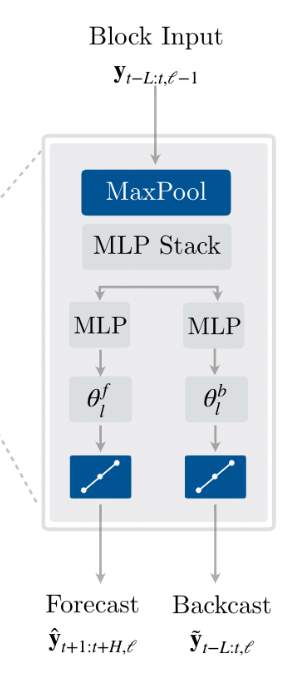
\includegraphics[width=1\textwidth]{N-HiTS Block Input.png}
    \caption{N-HiTS’s Block Input}
    \label{fig:1}
    \end{minipage}
    \begin{minipage}{0.50\textwidth}
    - Each block consists of multiple MLP (Multi-Layer Perceptron) layers. \par
    \textbf{Multi-Rate Signal Sampling:} Each block in the model uses a MaxPool layer with varying kernel sizes to analyze input components at different scales. Larger kernel sizes filter out high-frequency components, allowing the block to focus on long-term trends, which is crucial for long-horizon forecasting.
\begin{itemize}
    \item  \textbf{MaxPooling Operation:} 
\[
y_i^{(k)} = \max_{j \in \mathcal{W}_k} x_{i+j}
\]
Where:
\begin{itemize}
    \item $\begin{aligned}[t]
            y_i^{(k)} & \text{ is the output after MaxPooling.} \\
            \end{aligned}$
    \item $\begin{aligned}[t]
            k, x & \text{ is the input time series.} \\
            \end{aligned}$
    \item $\begin{aligned}[t]
            {W}_k & \text{ represents the window of size k.} \\
            \end{aligned}$
\end{itemize}
\end{itemize}
\begin{itemize}
    \item  \textbf{Non-Linear Activation Function:} 
\[
y = \sigma(Wx + b)
\]
Where: 
\begin{itemize}
    \item $\begin{aligned}[t]
            y & \text{ is the output.} \\
            \end{aligned}$
    \item $\begin{aligned}[t]
            \sigma & \text{ is a non-linear activation function.} \\
            \end{aligned}$
    \item $\begin{aligned}[t]
            W & \text{ is the weight matrix.} \\
            \end{aligned}$
    \item $\begin{aligned}[t]
            x & \text{ is the input.} \\
            \end{aligned}$
    \item $\begin{aligned}[t]
            b & \text{ is the bias vector.} \\
            \end{aligned}$
\end{itemize}
\end{itemize}
\begin{itemize}
    \item  \textbf{Forward Interpolation Coefficients:} 
\[
\alpha_t = f_{\text{forward}}(x_t; \theta_f)
\]
Where: 
\begin{itemize}
    \item $\begin{aligned}[t]
            \alpha_t & \text{ are the forward interpolation coefficients.} \\
            \end{aligned}$
    \item $\begin{aligned}[t]
            f_{\text{forward}} & \text{ is the non-linear function.} \\
            \end{aligned}$
    \item $\begin{aligned}[t]
            \theta_f & \text{ are its parameters.} \\
            \end{aligned}$
\end{itemize}
\end{itemize}
\begin{itemize}
    \item  \textbf{Backward Interpolation Coefficients:} 
\[
\beta_t = f_{\text{backward}}(x_t; \theta_b)
\]
Where: 
\begin{itemize}
    \item $\begin{aligned}[t]
            \beta_t & \text{ are the backward interpolation coefficients.} \\
            \end{aligned}$
    \item $\begin{aligned}[t]
            f_{\text{backward}} & \text{ is the non-linear function.} \\
            \end{aligned}$
    \item $\begin{aligned}[t]
            \theta_f & \text{ are its parameters.} \\
            \end{aligned}$
\end{itemize}
\end{itemize}
    \end{minipage}
\end{figure}

\section{Result}
\subsection{VNM}
    \begin{table}[h]
\centering
\resizebox{0.5\textwidth}{!}{%
\begin{tabular}{|c|c|c|c|c|}
    \hline
    \rowcolor{red!20} 
    \textbf{Model} & \textbf{Train - Test} & \textbf{RMSE} & \textbf{MAE} & \textbf{MAPE} \\ 
    \hline
    \multirow{3}{*}{ARIMA} & 7 - 3 & 5142.76 & 4317.65 & 6.38 \%\\
    \cline{2-5}
    & 8 - 2 & 4422.28 & 3186.73 & 4.47\% \\
    \cline{2-5}
    & \textbf{9 - 1 }&  \textbf{2131.86} & \textbf{1888.54} & \textbf{2.83 }\% \\
    \hline
    \multirow{3}{*}{LR} & 7 - 3 & 9306.12 & 8345.64 & 11.86 \%\\
    \cline{2-5}
    & 8 - 2 & 7934.74 & 7278.31 & 10.46\% \\
    \cline{2-5}
    & \textbf{9 - 1} & \textbf{5528.21} & \textbf{5191.77} & \textbf{7.67}\% \\
    \hline
    \multirow{3}{*}{Random Forest} & 7 - 3 & 5037.99 & 4219.43 & 6.24 \%\\
    \cline{2-5}
    & 8 - 2 & 4501.74 & 3273.07 & 4.59\% \\
    \cline{2-5}
    & \textbf{9 - 1} & \textbf{2192.07} & \textbf{1952.69} & \textbf{2.93}\% \\
    \hline
    \multirow{3}{*}{RNN} & 7 - 3 & 1115.36 & 934.08 & 1.37 \%\\
    \cline{2-5}
    & \textbf{8 - 2} & \textbf{945.01} &  \textbf{723.96} & \textbf{1.07}\% \\
    \cline{2-5}
    & 9 - 1 & 1086.61 & 903.13 & 1.37\% \\
    \hline
    \multirow{3}{*}{GRU} & 7 - 3 & 977.76 & 770.05 & 1.13\%\\
    \cline{2-5}
    & \textbf{8 - 2} & \textbf{826.06} & \textbf{610.95} & \textbf{0.9}\% \\
    \cline{2-5}
    & 9 - 1 & 737.1 & 601.2 & 0.91\% \\
    \hline
    \multirow{3}{*}{LSTM} & 7 - 3 & 1238.38 & 970.47 & 1.42 \%\\
    \cline{2-5}
    & \textbf{8 - 2} & \textbf{880.63} & \textbf{646.22} & \textbf{0.95}\% \\
    \cline{2-5}
    & 9 - 1 & 823.88 & 678.14 & 1.03\% \\
    \hline
    \multirow{3}{*}{N-HiTS} & 7 - 3 & 2330.46 & 1759.26 & 2.55 \%\\
    \cline{2-5}
    & \textbf{8 - 2} & \textbf{2095.59 }& \textbf{1502.00} & \textbf{2.18}\% \\
    \cline{2-5}
    & 9 - 1 & 2261.62 & 1674.35 & 2.43\% \\
    \hline
    \multirow{3}{*}{AR-MOS} & 7 - 3 & 10177.71 & 8990.69 & 13.27 \%\\
    \cline{2-5}
    & 8 - 2 & 4836.85 & 4259.13 & 6.22\% \\
    \cline{2-5}
    &\textbf{ 9 - 1 }& \textbf{4020.65 }& \textbf{3404.02 }& \textbf{5.12}\% \\
    \hline
\end{tabular}%
}
\end{table}
Based on the VNM dataset divided into train - test (7-3,8-2 and 9-1) in 8 models, we can see that the GRU model has the best prediction.
\subsection{SAB}
\resizebox{0.5\textwidth}{!}{%
   \begin{tabular}{|c|c|c|c|c|c|c|}
     \hline
     \rowcolor{red!20}
        \textbf{Model} & \textbf{Train - Test}  & \textbf{RMSE} & \textbf{MAE} & \textbf{MAPE} \\ 
     \hline
      \multirow{3}{*}{ARIMA} & 7 - 3 & 19230.53 & 15671.6 & 24.77 \%\\
      \cline{2-5}
     & 8 - 2 & 15338.05 & 12838.62 & 21.36\% \\
      \cline{2-5}
     & \textbf{9 - 1} & \textbf{4225.89} & \textbf{3554.24} & \textbf{6.22}\% \\
    \hline
      \multirow{3}{*}{LR} & 7 - 3 & 25626.47 & 23112.90 & 34.58 \%\\
      \cline{2-5}
     & 8 - 2 & 23326.41 & 22220.45 & 34.97\% \\
      \cline{2-5}
     & \textbf{9 - 1} & \textbf{19936.54} & \textbf{19260.65} & \textbf{32.91}\% \\
    \hline
     \multirow{3}{*}{Random Forest} & 7 - 3 & 19373.5 & 15805.76 & 24.97 \%\\
      \cline{2-5}
     & 8 - 2 & 15497.91 & 13018.04 & 21.64\% \\
      \cline{2-5}
     & \textbf{9 - 1} & \textbf{4227.39} & \textbf{3555.76} & \textbf{6.22}\% \\
     \hline
     \multirow{3}{*}{RNN} & \textbf{7 - 3} & \textbf{1088.79} & \textbf{787.37} & \textbf{1.18} \%\\
      \cline{2-5}
     & 8 - 2 & 1696.68 &  1385.48 & 2.32\% \\
      \cline{2-5}
     & 9 - 1 & 1132.65 & 872.82 & 1.53\% \\
    \hline
    \multirow{3}{*}{GRU} & 7 - 3 & 1658.03 & 1299.64 & 1.98 \%\\
      \cline{2-5}
     & 8 - 2 & 1397.82 & 1025.8 & 1.72\% \\
      \cline{2-5}
     & \textbf{9 - 1} & \textbf{1053.29} & \textbf{829.7}& \textbf{1.45}\% \\
     \hline
     \multirow{3}{*}{LSTM} & \textbf{7 - 3} & \textbf{2127.75} & \textbf{1644.73} & \textbf{2.47} \%\\
      \cline{2-5}
     & 8 - 2 & 2311.27 & 1808.84 & 3.02\% \\
      \cline{2-5}
     & 9 - 1 & 2497.91 & 2161.99 & 3.76\% \\
     \hline
     \multirow{3}{*}{N-HiTS} & \textbf{7 - 3} & \textbf{3015.43} & \textbf{2545.39} & \textbf{4.51} \%\\
      \cline{2-5}
     & 8 - 2 & 3036.10 & 2588.66 & 4.59\% \\
      \cline{2-5}
     & 9 - 1 & 3502.49 & 3045.01 & 5.39\% \\
       \hline
     \multirow{3}{*}{AR-MOS} & 7 - 3 & 29301.53 & 24257.74 & 38.11 \%\\
      \cline{2-5}
     & 8 - 2 & 20362.23 & 17228.47 & 28.58\% \\
      \cline{2-5}
     & \textbf{9 - 1} & \textbf{5656.46} & \textbf{4841.45} & \textbf{8.45}\% \\
     \hline
     \end{tabular}%
     }
     \\ Based on the SAB dataset divided into train - test (7-3, 8-2 and 9-1) in 8 models, we can see that the RNN model has the best prediction.
\subsection{MSN}
\resizebox{0.5\textwidth}{!}{%
    \begin{tabular}{|c|c|c|c|c|c|c|}
     \hline
     \rowcolor{red!20}
       \textbf{Model} & \textbf{Train - Test}  & \textbf{RMSE} & \textbf{MAE} & \textbf{MAPE} \\ 
     \hline
      \multirow{3}{*}{ARIMA} & 7 - 3 & 13291.52 & 11674.73 & 16.14 \%\\
      \cline{2-5}
     & 8 - 2 & 6898.68 & 5790.18 & 8.19\% \\
      \cline{2-5}
     & \textbf{9 - 1 }& \textbf{7405.47} & \textbf{5798.65} & \textbf{7.94}\% \\
    \hline
      \multirow{3}{*}{LR} & 7 - 3 & 51280.86 & 48549.36 & 66.47 \%\\
      \cline{2-5}
     & 8 - 2 & 42095.85 & 41200.62 & 58.46\% \\
      \cline{2-5}
     & \textbf{9 - 1} & \textbf{31812.22} & \textbf{31498.50} & \textbf{46.09}\% \\
    \hline
     \multirow{3}{*}{Random Forest} & 7 - 3 & 12807.81 & 11199.82 & 15.44 \%\\
      \cline{2-5}
     & 8 - 2 & 6948.47 & 5820.15 & 8.27\% \\
      \cline{2-5}
     & \textbf{9 - 1} & \textbf{6973.04} & \textbf{5355.6} & \textbf{7.33}\% \\
     \hline
     \multirow{3}{*}{RNN} & 7 - 3 & 1830.66 & 1433.74 & 2.00 \%\\
      \cline{2-5}
     & 8 - 2 & 1814.29 &  1383.41 & 2.03\% \\
      \cline{2-5}
     & \textbf{9 - 1} & \textbf{1619.01} & \textbf{1301.06} & \textbf{1.83}\% \\
    \hline
    \multirow{3}{*}{GRU} & \textbf{7 - 3} & \textbf{1666.65} & \textbf{1245.97} & \textbf{1.74 }\%\\
      \cline{2-5}
     & 8 - 2 & 1652.33 & 1248.06 & 1.83\% \\
      \cline{2-5}
     & 9 - 1 & 1617.84 & 1328.49 & 1.85\% \\
     \hline
     \multirow{3}{*}{LSTM} & 7 - 3 & 2885.91 & 2380.93 & 3.31 \%\\
      \cline{2-5}
     & 8 - 2 & 1774.21 & 1315.41 & 1.93\% \\
      \cline{2-5}
     & \textbf{9 - 1} & \textbf{1449.96} & \textbf{1179.24} & \textbf{1.65}\% \\
     \hline
     \multirow{3}{*}{N-HiTS} & \textbf{7 - 3} & \textbf{5295.94} & \textbf{4145.69} & \textbf{5.55} \%\\
      \cline{2-5}
     & 8 - 2 & 6820.29 & 5450.65 & 7.29\% \\
      \cline{2-5}
     & 9 - 1 & 7422.50 & 5974.11 & 7.99\% \\
       \hline
     \multirow{3}{*}{AR-MOS} & 7 - 3 & 12985.62 & 11387.46 & 15.77 \%\\
      \cline{2-5}
     & 8 - 2 & 7671.23 & 6350.45 & 9.1\% \\
      \cline{2-5}
     & \textbf{9 - 1} & \textbf{5601.88} & \textbf{4134.57} & \textbf{5.65}\% \\
     \hline
     \end{tabular}%
     }
     \\
     \\ Based on the MSN dataset divided into train - test (7-3,8-2 and 9-1) in 8 models, we can see that the LSTM model has the best prediction.
    \begin{figure}[H]
    \centering
    \begin{minipage}{0.23\textwidth}
    \centering
    \includegraphics[width=0.8\textwidth]{ARIMA model’s result for VNM with the rate of 7-3.png}
    \caption{ARIMA model’s result for VNM with the rate of 7-3}
    \end{minipage}
    \hfill
    \begin{minipage}{0.23\textwidth}
    \centering
    \includegraphics[width=0.8\textwidth]{ARIMA model’s result for VNM with the rate of 8-2.png}
    \caption{ARIMA model’s result for VNM with the rate of 8-2}
    \end{minipage}
\end{figure}
\begin{figure}[H]
    \begin{minipage}{0.23\textwidth}
    \centering
    \includegraphics[width=0.8\textwidth]{ARIMA model’s result for VNM with the rate of 9-1.png}
    \caption{ARIMA model’s result for VNM with the rate of 9-1}
    \end{minipage}
    \hfill
    \begin{minipage}{0.23\textwidth}
    \centering
    \includegraphics[width=0.8\textwidth]{ARIMA model’s result for SAB with the rate of 7-3.png}
    \caption{ARIMA model’s result for SAB with the rate of 7-3}

    \end{minipage}
   \end{figure}

   \begin{figure}[H]
    \centering
    \begin{minipage}{0.23\textwidth}
    \centering
    \includegraphics[width=0.8\textwidth]{ARIMA model’s result for SAB with the rate of 8-2.png}
    \caption{ARIMA model’s result for SAB with the rate of 8-2}
    \end{minipage}
    \hfill
    \begin{minipage}{0.23\textwidth}
    \centering
    \includegraphics[width=0.8\textwidth]{ARIMA model’s result for SAB with the rate of 9-1.png}
    \caption{ARIMA model’s result for SAB with the rate of 9-1}
    \end{minipage}
    \end{figure}
    \begin{figure}[H]
    \begin{minipage}{0.23\textwidth}
    \centering
    \includegraphics[width=0.8\textwidth]{ARIMA model’s result for MSN with the rate of 7-3.png}
    \caption{ARIMA model’s result for MSN with the rate of 7-3}
    \end{minipage}
    \hfill
    \begin{minipage}{0.23\textwidth}
    \centering
    \includegraphics[width=0.8\textwidth]{ARIMA model’s result for MSN with the rate of 8-2.png}
    \caption{ARIMA model’s result for MSN with the rate of 8-2}
    \end{minipage}
   \end{figure}

   \begin{figure}[H]
    \centering
    \begin{minipage}{0.23\textwidth}
    \centering
    \includegraphics[width=0.8\textwidth]{ARIMA model’s result for MSN with the rate of 9-1.png}
    \caption{ARIMA model’s result for MSN with the rate of 9-1}
    \end{minipage}
    \hfill
    \begin{minipage}{0.23\textwidth}
    \centering
    \includegraphics[width=0.8\textwidth]{LR model’s result for VNM with the rate of 7-3.png}
    \caption{LR model’s result for VNM with the rate of 7-3}
    \end{minipage}
    \end{figure}
    \begin{figure}[H]
    \begin{minipage}{0.23\textwidth}
    \centering
    \includegraphics[width=0.8\textwidth]{LR model’s result for VNM with the rate of 8-2.png}
    \caption{LR model’s result for VNM with the rate of 8-2}
    \end{minipage}
    \hfill
    \begin{minipage}{0.23\textwidth}
    \centering
    \includegraphics[width=0.8\textwidth]{LR model’s result for VNM with the rate of 9-1.png}
    \caption{LR model’s result for VNM with the rate of 9-1}
    \end{minipage}
   \end{figure}
   
   \begin{figure}[H]
    \centering
    \begin{minipage}{0.23\textwidth}
    \centering
    \includegraphics[width=0.8\textwidth]{LR model’s result for SAB with the rate of 7-3.png}
    \caption{LR model’s result for SAB with the rate of 7-3}
    \end{minipage}
    \hfill
    \begin{minipage}{0.23\textwidth}
    \centering
    \includegraphics[width=0.8\textwidth]{LR model’s result for SAB with the rate of 8-2.png}
    \caption{LR model’s result for SAB with the rate of 8-2}
    \end{minipage}
    \end{figure}
    
    \begin{figure}[H]
    \begin{minipage}{0.23\textwidth}
    \centering
    \includegraphics[width=0.8\textwidth]{LR model’s result for SAB with the rate of 9-1.png}
    \caption{LR model’s result for SAB with the rate of 9-1}
    \end{minipage}
    \hfill
    \begin{minipage}{0.23\textwidth}
    \centering
    \includegraphics[width=0.8\textwidth]{LR model’s result for MSN with the rate of 7-3.png}
    \caption{LR model’s result for MSN with the rate of 7-3}
    \end{minipage}
   \end{figure}

    \begin{figure}[H]
    \centering
    \begin{minipage}{0.23\textwidth}
    \centering
    \includegraphics[width=0.8\textwidth]{LR model’s result for MSN with the rate of 8-2.png}
    \caption{LR model’s result for MSN with the rate of 8-2}
    \end{minipage}
    \hfill
    \begin{minipage}{0.23\textwidth}
    \centering
    \includegraphics[width=0.8\textwidth]{LR model’s result for MSN with the rate of 9-1.png}
    \caption{LR model’s result for MSN with the rate of 9-1}
    \end{minipage}
     \end{figure}
  \begin{figure}[H]
    \centering
    \begin{minipage}{0.23\textwidth}
    \centering
    \includegraphics[width=0.8\textwidth]{Random Forest model’s result for VNM with the rate of 7-3.png}
    \caption{Random Forest model’s result for VNM with the rate of 7-3}
    \end{minipage}
    \hfill
    \begin{minipage}{0.23\textwidth}
    \centering
    \includegraphics[width=0.8\textwidth]{Random Forest model’s result for VNM with the rate of 8-2.png}
    \caption{Random Forest model’s result for VNM with the rate of 8-2}
    \end{minipage}

    \begin{minipage}{0.23\textwidth}
    \centering
    \includegraphics[width=0.8\textwidth]{Random Forest model’s result for VNM with the rate of 9-1.png}
    \caption{Random Forest model’s result for VNM with the rate of 9-1}
    \end{minipage}
    \hfill
    \begin{minipage}{0.23\textwidth}
    \centering
    \includegraphics[width=0.8\textwidth]{Random Forest model’s result for SAB with the rate of 7-3.png}
    \caption{Random Forest model’s result for SAB with the rate of 7-3}
    \end{minipage}
   \end{figure}

     \begin{figure}[H]
    \centering
    \begin{minipage}{0.23\textwidth}
    \centering
    \includegraphics[width=0.8\textwidth]{Random Forest model’s result for SAB with the rate of 8-2.png}
    \caption{Random Forest model’s result for SAB with the rate of 8-2}
    \end{minipage}
    \hfill
    \begin{minipage}{0.23\textwidth}
    \centering
    \includegraphics[width=0.8\textwidth]{Random Forest model’s result for SAB with the rate of 9-1.png}
    \caption{Random Forest model’s result for SAB with the rate of 9-1}
    \end{minipage}

    \begin{minipage}{0.23\textwidth}
    \centering
    \includegraphics[width=0.8\textwidth]{Random Forest model’s result for MSN with the rate of 7-3.png}
    \caption{Random Forest model’s result for MSN with the rate of 7-3}
    \end{minipage}
    \hfill
    \begin{minipage}{0.23\textwidth}
    \centering
    \includegraphics[width=0.8\textwidth]{Random Forest model’s result for MSN with the rate of 8-2.png}
    \caption{Random Forest model’s result for MSN with the rate of 8-2}
    \end{minipage}
   \end{figure}

    \begin{figure}[H]
    \centering
    \begin{minipage}{0.23\textwidth}
    \centering
    \includegraphics[width=0.8\textwidth]{Random Forest model’s result for MSN with the rate of 9-1.png}
    \caption{Random Forest model’s result for MSN with the rate of 9-1}
    \end{minipage}
    \begin{minipage}{0.23\textwidth}
    \centering
    \includegraphics[width=0.8\textwidth]{RNN model’s result for VNM with the rate of 7-3.png }
    \caption{RNN model’s result for VNM with the rate of 7-3}
    \end{minipage}
    \end{figure}

    \begin{figure}[H]
    \begin{minipage}{0.23\textwidth}
    \centering
    \includegraphics[width=0.8\textwidth]{RNN model’s result for VNM with the rate of 8-2.png }
    \caption{RNN model’s result for VNM with the rate of 8-2}
    \end{minipage}
    \begin{minipage}{0.23\textwidth}
    \centering
    \includegraphics[width=0.8\textwidth]{RNN model’s result for VNM with the rate of 9-1.png }
    \caption{RNN model’s result for VNM with the rate of 9-1}
    \end{minipage}
    \end{figure}
    
    \begin{figure}[H]
    \begin{minipage}{0.23\textwidth}
    \centering
    \includegraphics[width=0.8\textwidth]{RNN model’s result for SAB with the rate of 7-3.png }
    \caption{RNN model’s result for SAB with the rate of 7-3}
    \end{minipage}
    \hfill
    \begin{minipage}{0.23\textwidth}
    \centering
    \includegraphics[width=0.8\textwidth]{RNN model’s result for SAB with the rate of 8-2.png }
    \caption{RNN model’s result for SAB with the rate of 8-2}
    \end{minipage}
    \end{figure}
    
    \begin{figure}[H]
    \begin{minipage}{0.23\textwidth}
    \centering
    \includegraphics[width=0.8\textwidth]{RNN model’s result for SAB with the rate of 9-1.png }
    \caption{RNN model’s result for SAB with the rate of 9-1}
    \end{minipage}
     \hfill
     \begin{minipage}{0.23\textwidth}
    \centering
    \includegraphics[width=0.8\textwidth]{RNN model’s result for MSN with the rate of 7-3.png  }
    \caption{RNN model’s result for MSN  with the rate of 7-3}
    \end{minipage}
     \end{figure}
     
    \begin{figure}[H]
    \begin{minipage}{0.23\textwidth}
    \centering
    \includegraphics[width=0.8\textwidth]{RNN model’s result for MSN with the rate of 8-2.png }
    \caption{RNN model’s result for MSN with the rate of 8-2}
    \end{minipage}
     \hfill
     \begin{minipage}{0.23\textwidth}
    \centering
    \includegraphics[width=0.8\textwidth]{RNN model’s result for MSN with the rate of 9-1.png  }
    \caption{RNN model’s result for MSN  with the rate of 9-1}
    \end{minipage}
\end{figure}

   \begin{figure}[H]
    \begin{minipage}{0.23\textwidth}
    \centering
    \includegraphics[width=0.8\textwidth]{GRU model’s result for VNM with the rate of 7-3.png}
    \caption{GRU model’s result for VNM with the rate of 7-3}
    \end{minipage}
    \hfill
    \begin{minipage}{0.23\textwidth}
    \centering
    \includegraphics[width=0.8\textwidth]{GRU model’s result for VNM with the rate of 8-2.png}
    \caption{GRU model’s result for VNM with the rate of 8-2}
    \end{minipage}
    \end{figure}
    
    \begin{figure}[H]
    
    \begin{minipage}{0.23\textwidth}
    \centering
    \includegraphics[width=0.8\textwidth]{GRU model’s result for VNM with the rate of 9-1.png}
    \caption{GRU model’s result for VNM with the rate of 9-1}
    \end{minipage}   
   \hfill
    \centering
    \begin{minipage}{0.23\textwidth}
    \centering
    \includegraphics[width=0.8\textwidth]{GRU model’s result for SAB with the rate of 7-3.png}
    \caption{GRU model’s result for SAB with the rate of 7-3}
    \end{minipage}
     \end{figure}
     
     \begin{figure}[H]
    \begin{minipage}{0.23\textwidth}
    \centering
    \includegraphics[width=0.8\textwidth]{GRU model’s result for SAB with the rate of 8-2.png}
    \caption{GRU model’s result for SAB with the rate of 8-2}
    \end{minipage}
    \hfill
    \begin{minipage}{0.23\textwidth}
    \centering
    \includegraphics[width=0.8\textwidth]{GRU model’s result for SAB with the rate of 9-1.png}
    \caption{GRU model’s result for SAB with the rate of 9-1}
    \end{minipage}
    \end{figure}
    \begin{figure}[H]
    \begin{minipage}{0.23\textwidth}
    \centering
    \includegraphics[width=0.8\textwidth]{GRU model’s result for MSN with the rate of 7-3.png}
    \caption{GRU model’s result for MSN with the rate of 7-3}
    \end{minipage}   
    \hfill
    \begin{minipage}{0.23\textwidth}
    \centering
    \includegraphics[width=0.8\textwidth]{GRU model’s result for MSN with the rate of 8-2.png}
    \caption{GRU model’s result for MSN with the rate of 8-2}
    \end{minipage}
    \end{figure}
    
   \begin{figure}[H]

    \begin{minipage}{0.23\textwidth}
    \centering
    \includegraphics[width=0.8\textwidth]{GRU model’s result for MSN with the rate of 9-1.png}
    \caption{GRU model’s result for MSN with the rate of 9-1}
    \end{minipage}
    \hfill
    \begin{minipage}{0.23\textwidth}
    \centering
    \includegraphics[width=0.8\textwidth]{LSTM model’s result for MSN with the rate of 7-3.png}
    \caption{LSTM model’s result for MSN with the rate of 7-3}
    \end{minipage}
    \end{figure}
    
    \begin{figure}[H]

    \begin{minipage}{0.23\textwidth}
    \centering
    \includegraphics[width=0.8\textwidth]{LSTM model’s result for MSN with the rate of 8-2.png}
    \caption{LSTM model’s result for MSN with the rate of 8-2}
    \end{minipage}
    \hfill
    \begin{minipage}{0.23\textwidth}
    \centering
    \includegraphics[width=0.8\textwidth]{LSTM model’s result for MSN with the rate of 9-1.png}
    \caption{LSTM model’s result for MSN with the rate of 9-1}
    \end{minipage}
    \end{figure}
    \begin{figure}[H]
    \begin{minipage}{0.23\textwidth}
    \centering
    \includegraphics[width=0.8\textwidth]{LSTM model’s result for SAB with the rate of 7-3.png}
    \caption{LSTM model’s result for SAB with the rate of 7-3}
    \end{minipage}
    \hfill
    \begin{minipage}{0.23\textwidth}
    \centering
    \includegraphics[width=0.8\textwidth]{LSTM model’s result for SAB with the rate of 8-2.png}
    \caption{LSTM model’s result for SAB with the rate of 8-2}
    \end{minipage}
    \end{figure}
    
    \begin{figure}[H]
    \begin{minipage}{0.23\textwidth}
    \centering
    \includegraphics[width=0.8\textwidth]{LSTM model’s result for SAB with the rate of 9-1.png}
    \caption{LSTM model’s result for SAB with the rate of 9-1}
    \end{minipage}
    \hfill
    \begin{minipage}{0.23\textwidth}
    \centering
    \includegraphics[width=0.8\textwidth]{LSTM model’s result for VNM with the rate of 7-3.png }
    \caption{LSTM model’s result for VNM with the rate of 7-3}
    \end{minipage}
    \end{figure}

    \begin{figure}[H]
    \begin{minipage}{0.23\textwidth}
    \centering
    \includegraphics[width=0.8\textwidth]{LSTM model’s result for VNM with the rate of 8-2.png}
    \caption{LSTM model’s result for VNM with the rate of 8-2}
    \end{minipage}
    \hfill
    \begin{minipage}{0.23\textwidth}
    \centering
    \includegraphics[width=0.8\textwidth]{LSTM model’s result for VNM with the rate of 9-1.png }
    \caption{LSTM model’s result for VNM with the rate of 9-1}
    \end{minipage}
    \end{figure}

    \begin{figure}[H]
    \begin{minipage}{0.23\textwidth}
    \centering
    \includegraphics[width=0.8\textwidth]{N-HiTS model’s result for VNM with the rate of 7-3.png}
    \caption{N-HiTS model’s result for VNM with the rate of 7-3}
    \end{minipage}
    \hfill
    \begin{minipage}{0.23\textwidth}
    \centering
    \includegraphics[width=0.8\textwidth]{N-HiTS model’s result for VNM with the rate of 8-2.png }
    \caption{N-HiTS model’s result for VNM with the rate of 8-2}
    \end{minipage}
    \end{figure}

    \begin{figure}[H]
    \begin{minipage}{0.23\textwidth}
    \centering
    \includegraphics[width=0.8\textwidth]{N-HiTS model’s result for VNM with the rate of 9-1.png}
    \caption{N-HiTS model’s result for VNM with the rate of 9-1}
    \end{minipage}
    \hfill
    \begin{minipage}{0.23\textwidth}
    \centering
    \includegraphics[width=0.8\textwidth]{N-HiTS model’s result for SAB with the rate of 7-3.png }
    \caption{N-HiTS model’s result for SAB with the rate of 7-3}
    \end{minipage}
    \end{figure}

    \begin{figure}[H]
    \begin{minipage}{0.23\textwidth}
    \centering
    \includegraphics[width=0.8\textwidth]{N-HiTS model’s result for SAB with the rate of 8-2.png}
    \caption{N-HiTS model’s result for SAB with the rate of 8-2}
    \end{minipage}
    \hfill
    \begin{minipage}{0.23\textwidth}
    \centering
    \includegraphics[width=0.8\textwidth]{N-HiTS model’s result for SAB with the rate of 9-1.png }
    \caption{N-HiTS model’s result for SAB with the rate of 9-1}
    \end{minipage}
    \end{figure}

    \begin{figure}[H]
    \begin{minipage}{0.23\textwidth}
    \centering
    \includegraphics[width=0.8\textwidth]{N-HiTS model’s result for MSN with the rate of 7-3.png}
    \caption{N-HiTS model’s result for MSN with the rate of 7-3}
    \end{minipage}
    \hfill
    \begin{minipage}{0.23\textwidth}
    \centering
    \includegraphics[width=0.8\textwidth]{N-HiTS model’s result for MSN with the rate of 8-2.png }
    \caption{N-HiTS model’s result for MSN with the rate of 8-2}
    \end{minipage}
    \end{figure}

    \begin{figure}[H]
    \begin{minipage}{0.23\textwidth}
    \centering
    \includegraphics[width=0.8\textwidth]{N-HiTS model’s result for MSN with the rate of 9-1.png}
    \caption{N-HiTS model’s result for MSN with the rate of 9-1}
    \end{minipage}
    \hfill
    \begin{minipage}{0.23\textwidth}
    \centering
    \includegraphics[width=0.8\textwidth]{AR-MOS model’s result for VNM with the rate of 7-3.png }
    \caption{AR-MOS model’s result for VNM with the rate of 7-3}
    \end{minipage}
    \end{figure}
    
    \begin{figure}[H]
    \begin{minipage}{0.23\textwidth}
    \centering
    \includegraphics[width=0.8\textwidth]{AR-MOS model’s result for VNM with the rate of 8-2.png}
    \caption{AR-MOS model’s result for VNM with the rate of 8-2}
    \end{minipage}
    \hfill
    \begin{minipage}{0.23\textwidth}
    \centering
    \includegraphics[width=0.8\textwidth]{AR-MOS model’s result for VNM with the rate of 9-1.png }
    \caption{AR-MOS model’s result for VNM with the rate of 9-1}
    \end{minipage}
    \end{figure}
    
    \begin{figure}[H]
    \begin{minipage}{0.23\textwidth}
    \centering
    \includegraphics[width=0.8\textwidth]{AR-MOS model’s result for SAB with the rate of 7-3.png}
    \caption{AR-MOS model’s result for SAB with the rate of 7-3}
    \end{minipage}
    \hfill
    \begin{minipage}{0.23\textwidth}
    \centering
    \includegraphics[width=0.8\textwidth]{AR-MOS model’s result for SAB with the rate of 8-2.png}
    \caption{AR-MOS model’s result for SAB with the rate of 8-2}
    \end{minipage}
    \end{figure}
    
    \begin{figure}[H]
    \begin{minipage}{0.23\textwidth}
    \centering
    \includegraphics[width=0.8\textwidth]{AR-MOS model’s result for SAB with the rate of 9-1.png}
    \caption{AR-MOS model’s result for SAB with the rate of 9-1}
    \end{minipage}
    \hfill
    \begin{minipage}{0.23\textwidth}
    \centering
    \includegraphics[width=0.8\textwidth]{AR-MOS model’s result for MSN with the rate of 7-3.png }
    \caption{AR-MOS model’s result for MSN with the rate of 7-3}
    \end{minipage}
    \end{figure}

    \begin{figure}[H]
    \begin{minipage}{0.23\textwidth}
    \centering
    \includegraphics[width=0.8\textwidth]{AR-MOS model’s result for MSN with the rate of 8-2.png}
    \caption{AR-MOS model’s result for MSN with the rate of 8-2}
    \end{minipage}
    \hfill
    \begin{minipage}{0.23\textwidth}
    \centering
    \includegraphics[width=0.8\textwidth]{AR-MOS model’s result for MSN with the rate of 9-1.png }
    \caption{AR-MOS model’s result for MSN with the rate of 9-1}
    \end{minipage}
    \end{figure}
   \section{CONCLUSION}
Among the eight algorithms (Linear Regression, ARIMA, RNN, GRU, LSTM, AR-MOS, Random Forest, N-HiTS), the results of this study show that the RNN, GRU, and LSTM models are the most suitable for predicting the stock prices of three corporations: VNM, SAB, and MSN. In contrast, other models (ARIMA, Linear Regression, Random Forest, N-HiTS, AR-MOS) did not perform as well. This study emphasizes the necessity of employing multiple modeling approaches in financial analysis and highlights the potential of using RNN, GRU, and LSTM models for stock price prediction in the future. Through assessment of strengths and weaknesses of these models, we aim to provide valuable guidance to investors, traders and researchers in choosing the appropriate forecasting model to predict stock prices.

Based on these findings, further research on model tuning and optimization techniques could yield even better predictive performance. Exploring various advanced architectures can improve accuracy. Testing models across different markets and sectors will assess their robustness and generalizability. By following this development, researchers and practitioners can develop more complex, reliable and effective stock price prediction models. Continued innovation and research in this field are essential for developing more robust and accurate predictive tools.

 \section{ACKNOWLEDGMENT}
   Our team would like to express our deepest gratitude to \textbf{PhD. Nguyen Dinh Thuan}  and \textbf{Mr. Nguyen Minh Nhut}, whose guidance and support helped us successfully complete this project. Despite our best efforts to apply what we have learned, it is difficult to avoid mistakes entirely. Therefore, we look forward to receiving feedback from our instructors to improve and refine our work. This feedback will help us accumulate knowledge and experience, preparing us better for the future.
%% UNCOMMENT these lines below (and remove the 2 commands above) if you want to embed the bibliografy.
\begin{thebibliography}{00}
\bibitem{b1} Avijeet Biswal, “Stock Market Prediction using Machine Learning in 2024”, Apr. 15, 2024
\bibitem{b2} V. Gururaj, ”Stock Market Prediction using Linear Regression and Support Vector Machines” vol. 14, no. 8, 2019.

\bibitem{b3} Adam Hayes, “Autoregressive Integrated Moving Average (ARIMA) Prediction Model”, April 05, 2024
https://www.investopedia.com/terms/a/autoregressive-integrated-moving-average-arima.asp
\bibitem{b4} Aayush Bajaj, “ARIMA and SARIMA: Real-World Time Series Forecasting”, Aug. 18th, 2023.
https://neptune.ai/blog/arima-sarima-real-world-time-series-forecasting-guide
\bibitem{b5} Robert Nau, Duke University, Fuqua School of Business. "Introduction to ARIMA: Nonseasonal Models”
https://people.duke.edu/~rnau/411arim.htm
\bibitem{b6} Hyndman, R.J., and Athanasopoulos, G. (2018) Forecasting: principles and practice, 2nd edition, OTexts: Melbourne, Australia. 
\bibitem{b7} What Is Linear Regression? | IBM.
\bibitem{b8} Multiple Linear Regression (MLR) Definition, Formula, and Example (investopedia.com).
\bibitem{b9} https://www.geeksforgeeks.org/autoregressive-ar-model-for-time-series-forecasting/
https://arxiv.org/pdf/2402.00555v1
\bibitem{b10} Sruthi ER, “Understand Random Forest Algorithms With Examples”
https://www.analyticsvidhya.com/blog/2021/06/understanding-random-forest/
\bibitem{b11} IBM, “What is random forest?”, Last updated: Feb. 22, 2024.
\bibitem{b12} https://www.geeksforgeeks.org/introduction-to-recurrent-neural-network/
\bibitem{b13} https://community.arm.com/arm-community-blogs/b/ai-and-ml-blog/posts/rnn-models-ethos-u
\bibitem{b14}  https://www.simplilearn.com/tutorials/deep-learning-tutorial/rnn
\bibitem{b15}https://www.geeksforgeeks.org/understanding-of-lstm-networks/
\bibitem{b16}https://www.analyticsvidhya.com/blog/2022/03/an-overview-on-long-short-term-memory-lstm/
\bibitem{b17}“Gated Recurrent Unit,” DeepAI, May 17, 2019 https://deepai.org/machine-learning-glossary-and-terms/gated-recurrent-unit
\bibitem{b18}“Gated Recurrent Unit Networks”, GeekforGeeks, Mar. 02, 2023 https://www.geeksforgeeks.org/gated-recurrent-unit-networks/
\bibitem{b19} "Autoregressive Extensions of EMOS with
Application to Surface Temperature Ensemble
Postprocessing,19. April 2024.https://presentations.copernicus.org/EGU24/EGU24-4357_presentation.pdf"
\bibitem{b20} “Random Forest Algorithm”, https://www.javatpoint.com/machine-learning-random-forest-algorithm
\bibitem{b21}Tanushree Biswal, “Random Forest for Time Series Forecasting”, Last updated: Feb. 26, 2024
https://www.analyticsvidhya.com/blog/2021/06/random-forest-for-time-series-forecasting/
\bibitem{b22}GeeksforGeeks, “Random Forest for Time Series Forecasting”, Last Updated : 01 Nov, 2023 https://www.geeksforgeeks.org/random-forest-for-time-series-forecasting-using-r/

\end{thebibliography}
%%%%%%%%%%%%%%%


\EOD

\end{document}
